\documentclass[10pt]{article}
\usepackage[margin=0.4in]{geometry}
\usepackage{amsmath}
\usepackage{enumitem}
\usepackage{multicol}
\usepackage{tikz}
\usetikzlibrary{shapes.geometric}
\usepackage{soul}

\newcommand{\ds}{\displaystyle}
\newcommand{\on}{\operatorname}


\begin{document}
\newcounter{enumCount}
\pagestyle{empty}
\subsection*{Homework 9 - Math 140 \hfill Name: \underline{\hspace*{2in}}}


\noindent
\textit{Calculate the following derivatives.}
\begin{multicols}{2}
\begin{enumerate}
\item $\ds \frac{d}{dx} \dfrac{x}{x-2}$ 


\item $\ds \frac{d}{dy} e^{-5y}$ 

\setcounter{enumCount}{\theenumi}
\end{enumerate} 
\end{multicols}

\vfill


\begin{multicols}{2}
\begin{enumerate}
\setcounter{enumi}{\theenumCount}
\item $\ds \dfrac{d}{dx} \dfrac{1}{x^2 + 5x + 6}$.


\item $\ds \dfrac{d}{dx} \, (e^x + x^2)^5$.


\setcounter{enumCount}{\theenumi}
\end{enumerate} 
\end{multicols}
\vfill

\begin{multicols}{2}
\begin{enumerate}
\setcounter{enumi}{\theenumCount}
\item $\ds \dfrac{d}{dx} x e^{-x^2}$.


\item $\ds \dfrac{d}{dx} \, \dfrac{2e^x}{x^2}$.


\setcounter{enumCount}{\theenumi}
\end{enumerate} 
\end{multicols}
\vfill


\begin{multicols}{2}
\begin{enumerate}
\setcounter{enumi}{\theenumCount}
\item $\ds \dfrac{d}{dx} \ln(x^2 + 4 x)$.


\item $\ds \dfrac{d}{du} \, (e^{u}+1)^{-1}$.


\setcounter{enumCount}{\theenumi}
\end{enumerate} 
\end{multicols}
\vfill

\newpage

\noindent
\begin{enumerate}
\setcounter{enumi}{\theenumCount}

%\item The price elasticity of demand is given by the formula $\ds E = \left| \frac{p Q'}{Q} \right|.$
%Suppose that a business estimates that their customers will purchase $Q(p) = 400-10p$ items, when the price of each item is $p$ dollars.  What is the elasticity of demand when $p = \$10$? Is demand elastic or inelastic at that price?
%  \vfill
%  \vfill


\item A cup of hot water is set out to cool.  Its temperature (in Fahrenheit) is $T(t) = 70 + 80 e^{-0.1t}$ where $t$ is the time since it was set out, in minutes. 

\begin{enumerate}
\item  What is the derivative of the temperature function?
\vfill 

\item Use a calculator to find $T'(4)$. Explain clearly what this value tells us about the rate of change in temperature. 
\vfill
\end{enumerate}

\item Find the x-value where the tangent of the function $f(x) = 4 e^{-x}+x$ has slope equal to zero.
\begin{flushright}
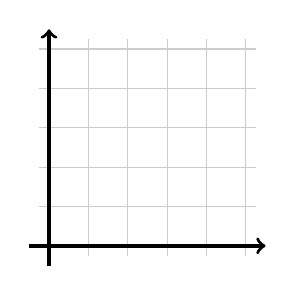
\begin{tikzpicture}[scale=0.5]
\draw[gray!40] (-0.25,-0.25) grid (5.25,5.25);
\draw[very thick,->] (-0.5,0) -- (5.5,0);
\draw[very thick,->] (0,-0.5) -- (0,5.5);
\draw[very thick,color=blue] plot[domain=-0.25:5,samples=400] function {4*exp(-x)+x};
\end{tikzpicture}
\end{flushright}
\vfill
\vfill
\vfill



\setcounter{enumCount}{\theenumi}
\end{enumerate}


\end{document}
